% vim: set fenc=utf-8 ft=latex encoding=utf-8
% -*- mode: latex; coding: UTF-8; -*-
%!TEX root = knowledge-curation.tex
\section{Methodology}
\label{cha:methodology}

The main goal of our study is to empirically compare how knowledge, specifically knowledge manifested as questions-and-answers, is seeked, shared, and curated in both, the \RH mailing list and the R section of \SO. We apply a qualitative \textit{exploratory case study} methodology~\cite{Creswell2009,Runeson2012} to answer the following research questions:
    \begin{enumerate}[label=\bfseries{RQ-\arabic*.},itemsep=3pt, topsep=2pt, leftmargin=3em, parsep=0pt]
        \item \rqa
        \item \rqb
        \item \rqc
     \end{enumerate}

%We performed a qualitative case study~\cite{Creswell2009,Runeson2012} of the knowledge that flows through both \RH and \SO.
%This research method is applicable when a concept or phenomenon requires more understanding, with little pre-existing research~\cite{Creswell2009}.

This study employs two research methods, \textit{mining archival data} and a \textit{qualitative survey}, and is composed of two phases. In the first phase, we conduct a random sampling of questions in both channels. Its purpose is to characterize the types of discussions that happen in both channels. We sampled 400 questions in each channel; this sample guaranteed both saturation and a reliability of 95\% $\pm$ 5\%. \alexey{How? more details on saturation.} In the second phase, we survey the members of the R-community to validate our interpretation of the results of the previous phase. %obtain further additional insights and to verify our findings.

\subsection{Phase I: mining archival data} 
\label{sec:studyDesign}

In this phase we mined both: the archives of the \RH mailing list and \SO archival data.

\subsubsection{Data collection and preparation}
\label{subsec:preparation}

We used the publicly available archives of both	the R-help mailing list and Stack Overflow. The R-Users mailing list dates started in 1997, while the archives for Stack Overflow start in 2008 (when it was created).
To make both data sets comparable, we analysed both datasets from 2008 until 2013, a period of time that both channels were available.
For Stack Overflow, we obtained a data dump file available on its website---Stack Exchange releases a new data dump from all their websites every three months\footnote{\url{http://stackexchange.com/sites}}. For the R-help mailing list data, we retrieved the archives available as MBOX files from the R website.

%To make the data comparable againt the Stack Overflow dat set, we transformed the email addresses to MD5 hashes, and changed the time zone of the mailing list messages (UTC+2) to the time zone used by Stack Overflow (UTC).
    
In order to answer RQ3 we needed the ability to compare email addresses between both channels. However, the last Stack Exchange dump file that contains email addresses as MD5 hashes was released in September 2013.
Since then, Stack Exchange does not provide the information about email addresses.
Because of this, we used the data dump file from September 2014, but updated the \texttt{users} table with the hashes taken from the September 2013 dump file, for whose \texttt{ID}s were identical in both data sets.
If a user from the 2013 data file did not exist in the 2014 data, we did not count it.
From \SO we retrieved all R-related data by selecting only messages with the R tag (\texttt{r}) and its synonyms\footnote{\url{http://stackoverflow.com/tags/r/synonyms}} (\texttt{rstats} and \texttt{r-language}).

To determine users who were active in both channels we compared the MD5 hashes of the R-Users participants to the MD5s hashes of the \SO participants. Given the limitations of the \SO data, we did not perform any unification of email addresses, and therefore consider every email address to belong to an independent individual. In total, we found 1,421 different users (email addresses) on both media channels.

    % Although MD5 hashes are not \textit{collision resistant} and could possibly lead to false positives, it is unlikely that two different email addresses share a MD5 hash.

We used two different software tools to prepare the data:
    \begin{enumerate*}[label=(\arabic*)]
    \item to process the Stack Overflow data, we used a modified version of Sam Saffron's application, So-Slow\footnote{\url{https://github.com/SamSaffron/So-Slow}}; and,
    \item to process the R-help mailing list archives, we wrote a our own mail mining application\footnote{Our tool is available at
            \url{https://github.com/cagomezt/GTMail}}, To ensure accurate results when processing the R-help mailing list, we followed the series of recommendations proposed by Bettenburg \textit{et al}.~\cite{Bettenburg2009}.
    \end{enumerate*}
Table~\ref{table:data} depicts a summary of the data used for this study. Unsurprisingly, the R-help mailing list has more questions, answers, and users, as it contains approximately ten years of additional data.
Note that only Stack Overflow's data contains ``comments'' information.

	\begin{table}[!htb]
	  \centering
      \caption{Raw data collected for each channel.}
      \begin{small}
        \begin{tabular}{lrr}
	        \toprule
	        Type          &  R-help & Stack Overflow \\
	        \midrule
	        Questions     & 101,931 &  67,393 \\
	        Answers       & 213,366 &  99,620 \\
	        Comments      &       - & 286,124 \\
	        Users         &  39,150 &  26,324 \\
	        \bottomrule
        \end{tabular}
      \end{small}
	  \label{table:data}
	\end{table}





\subsubsection{Data analysis process}
\label{sec:dap}

We followed an inductive approach~\cite{Runeson2012} to analyse the data from Stack Overflow and the R-help mailing list. This is an iterative process, where \alexey{missing word here?} across the study is necessary to switch between data selection and data analysis, or between data reporting and data collection. To reduce the risk of bias~\cite{Runeson2012}, two researchers conducted the analysis, both computer scientists with a background in qualitative data analysis. To answer RQ-1 and RQ-2, we selected 400 random threads of each channels. To answer RQ-3, we focused on questions that were posted with the same subject, sent to both channels, and by the same author. We found 79 such threads and analyzed them all.
    
    \begin{figure*}[htbp]
    	\centering
    	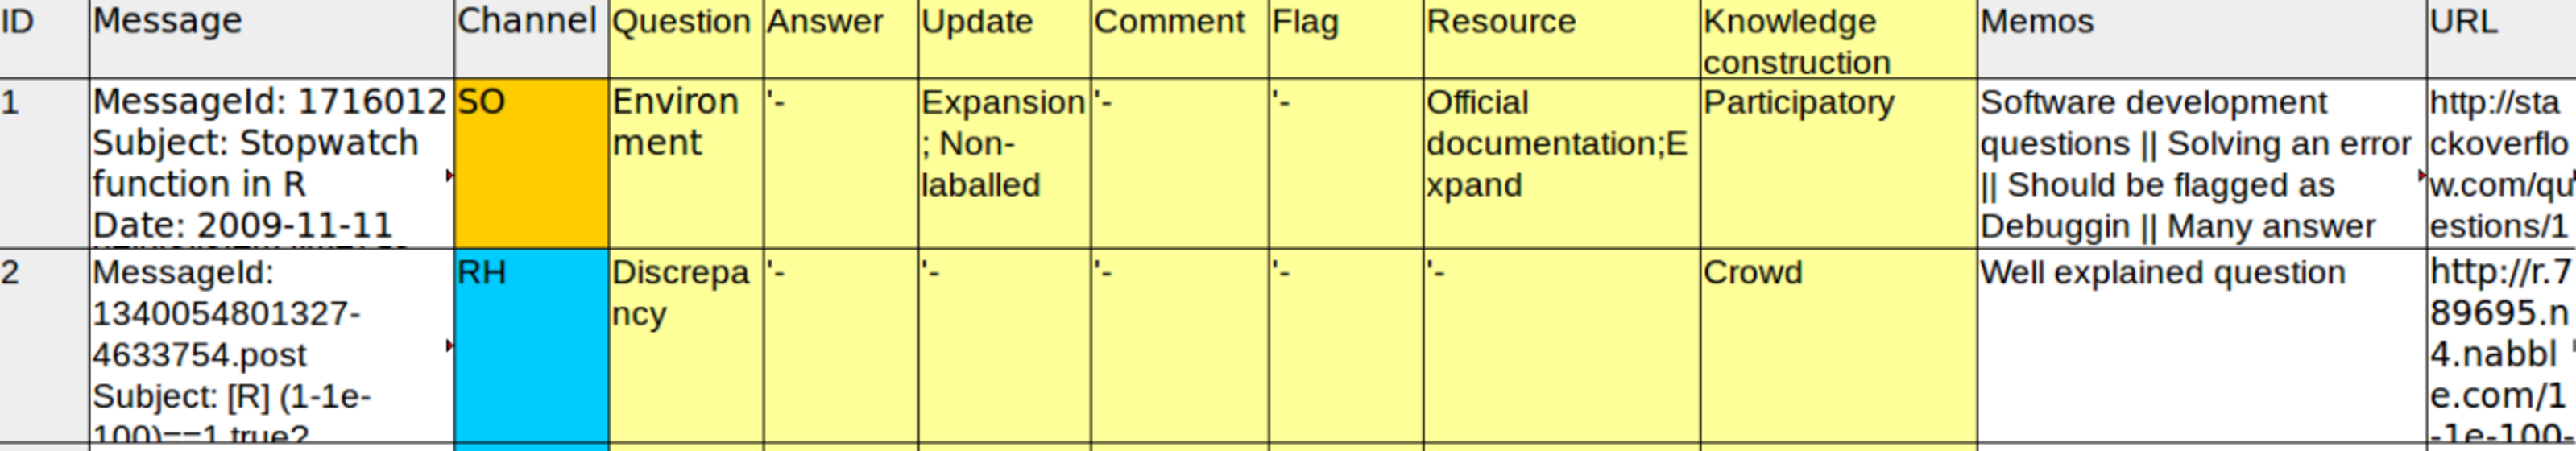
\includegraphics[width=.95\textwidth]{Figures/CodingExample}
    	\caption{Example of data coding. Each row is a thread message. Questions, comments, and answers are identified with the number on the first column. Columns in yellow contain the codification for each message type. The last two columns contain the memos and the URL.}
    	\label{fig:CodingExample}
%\vspace{-3mm}
    \end{figure*}

We used \textbf{memoing}, \textbf{affinity diagrams}, and a \textbf{code book} to support the data analysis process. We wrote reflective memos in a spreadsheet next to the applicable codes (see example in Fig.~\ref{fig:CodingExample}). These memos were used to create the codes and hypotheses about the relationships between concepts. We coded in multiple sessions, which allowed us to refine the code book definitions. Each entry is associated with a title, a formal definition, an example, and notes from the researcher. %The final version of the code book is detailed in section~\ref{cha:findings}.
For inter-rater reliability we used the Cohen Kappa \textbf{inter-rater agreement} coefficient~\cite{Stemler2004}. Although it is suggested to aim for coefficient values above 0.6 to obtain substantial results~\cite{Landis1977}, based on our previous experience with this method, we aimed for 0.8 or above. We used this coefficient after each coding session as a way to trigger discussion.



	% \begin{description}[itemsep=2pt, topsep=0pt, leftmargin=1em, parsep=0pt]
	% 	\item[Memoing] is the act of taking notes (coding) on what the researcher is learning from the data during the analysis~\cite{Groenewald2008}.
 %        We wrote reflective memos in a spreadsheet next to the applicable codes (see figure \ref{fig:CodingExample}).
 %        These memos were used to create the codes, and hypotheses about the relationships between concepts.

	% 	\item[Affinity diagrams] allows to organize ideas and data into groups, and to find the relationships between concepts~\cite{Scupin1997}.
	% 	We used them to discuss new insights, and while defining categories and relationships between them.

	% 	\item[Inter-rater agreement \textit{Cohen Kappa}] is a coefficient used to measure the agreement between two coders who classify items into mutually exclusive categories~\cite{Stemler2004}.
	% 	Ladis and Koch suggest that values above 0.60 or 60\% to obtain substantial results~\cite{Landis1977}.
	% 	In a previous study~\cite{Gomez2013}, we used the same coefficient to measure agreement between coders.
	% 	Based on this experience, we set a value above 0.80 or 80\% as the minimum to obtain substantial results.
	% 	We used this coefficient after each coding session as a way to trigger discussion.

	% 	\item[Code book] is a book that contains the definitions of the codes that researchers look during the data analysis~\cite{MacQueen1998}.
	% 	We coded in multiple sessions, which allowed us to refine the definitions.
	% 	Each entry is associated with a title, a formal definition, an example, and space for notes from the researcher.
	% 	The final version of the code book is detailed in section~\ref{cha:findings}.
	% \end{description}

The analysis process required an \textit{understanding of the context} surrounding each message. The process consisted of: (1) gathering the required information from both channels---i.e., the message analysed, and the relevant thread, and (2) mapping between messages from each channel to a specific knowledge type (see Section~\ref{cha:findings-types}). The mapping is necessary as each channel contains a different data structure.

For mapping R-help mailing list messages we defined the following:

	\begin{description}[itemsep=1pt, topsep=2pt, leftmargin=1em, parsep=0pt]
		\item[Question:] the message is the first on the thread, and it contains the main question.
		\item[Answer:] the message provides a solution to the main question of the thread.
	 	\item[Update:] the message claims for a modification to a question (or answer) made by the author of such a question (or answer).
		\item[Comment:] the message offers a clarification to a specific part of the question or answer.
		\item[Flag:] the message requests attention from the moderator (e.g., repeated questions, spam, or rude behaviour).
	\end{description}

%	The data set was capped at 400 threads for each channel when we deemed our observations as being saturated.

\subsection{Phase II: The survey} 

\alexey{do we use this data in any way in our paper? if not, we need either to use it or remove.}

    We conducted a survey\footnote{A copy of the survey is available at \url{http://goo.gl/mxmH5J}} with members of the R community with the purpose of obtaining additional insights on the findings.
    To test and refine the questions, format and tone, we performed two pilots.
    
    We announced our survey on Twitter, Reddit, the R-help mailing list, and Meta Stack Exchange to reach users of both channels, and minimize the selection bias.
    However, on Stack Exchange the was deemed out of topic and was deleted a few minutes later. We received 26 valid responses.

%%% Local Variables:
%%% mode: latex
%%% TeX-master: "knowledge-curation.tex"
%%% End:
